\section{Development and Implementation}

Whilst the full source code is available in the appendix, the following section contains the most important parts of the code-base, highlighting the techniques used and technical solutions employed.

\subsection{Summary of techniques}
For handy reference, below is a table summarising the various techniques used in the codebase. \textbf{These are expanded upon in more detail below}.

{
	\renewcommand{\arraystretch}{1.5}
	\begin{table}[h!]
		\begin{center}
			\begin{tabularx}{1.0 \textwidth} {
					| >{\raggedright\arraybackslash}X 
					| >{\raggedright\arraybackslash}X
					| >{\raggedright\arraybackslash}X 
					|
				}
				\hline
				Source File & Technique & Purpose \\
				
				\hline
				include/data/atomic\_linked\_list.h & Thread-safe linked list (including linked list maintenance) from scratch and use of function callbacks & Provides data structure for inter-thread communication (see section 2.1) \\
				
				\hline
				include/data/tree.h and src/ui/file\_browser.cpp & Tree data structure and recursive navigation of filesystem & Used in file browsing to represent filesystem structure and allow the user to browse for audio files \\
				
				\hline
				src/data/merge-sort.cpp & Recursive merge-sort  algorithm implementation & To sort playlist files alphabetically \\
				
				\hline
				src/effects/fft.cpp & Cooley-Tukey Fast Fourier algorithm implementation & To aid in audio procession and visualisation \\
				
				\hline
				src/ui/audio\_visualiser.cpp & Uses FFT data & Renders audio visualisation \\
				
				\hline
				include/effects/audio\_effect.cpp & Polymorphic "audio effect" base class (inherited by children) - including use of hashmap & Manages common interface \\
				
				\hline
				src/effects/echo\_effect.cpp & Inheritance & Echo effect implementation \\
				
				\hline
				src/effects/equaliser\_effect.cpp &  Inheritance and use of Fourier algorithms & Audio equaliser implementation \\
				
				\hline
				src/effects/noise\_effect.cpp & Inheritance & Noise effect implementation \\
				
				\hline
				src/effects/volume\_effect.cpp & Inheritance & Volume effect implementation \\
				
				\hline
				Various files & Use of function callbacks & Used in many places, including preset creation and UI code \\
				
				\hline
				Various files & Error handling and user input sanitisation & Prevent program from experiencing crashes, security issues and undefined behaviour \\
				
				\hline
			\end{tabularx}
		\end{center}
	\end{table}
}

\pagebreak
\subsection{Atomic Linked List - \textit{include/data/atomic\_linked\_list.h}}
As discussed in section 2, the atomic linked list is a crucial component of the project.  It makes use of generics (C++ "templates") to allow it to store any arbitrary data type. 

The full code is listed below, followed by explanations below of the most critical parts.

\inputminted[linenos]{c++}{../include/data/atomic_linked_list.h}

\paragraph{Mutexes} Whenever a caller accesses the data structure, the mutex is first locked. The relevant operation is then performed, and the mutex is then unlocked, freeing the data structure for future use (in this thread or otherwise). This can be seen in the functions Add, Remove, ForEach, SwapWithNext and Reset.

\paragraph{Generics} To make the data structure as flexible as possible, it is written to store a generic type "T". Note that we cannot store a variable of type T directly, but must rather store a pointer to each "T", as some types may be too big to store on the stack.

\paragraph{Callbacks} The data structure provides a "ForEach" method which takes a callback as an argument. This callback is invoked upon every node in the linked list, in order to allow for arbitrary operations to be formed on each element. This is used in \textit{src/io/audio\_stream.cpp} and \textit{src/ui/effects\_window.cpp} to iterate over each node. For example, in the \textit{AudioStream} class:
\begin{minted}{c++}
effects->ForEach([&](AudioEffect* effect) {
	effect->ApplyEffect(packet);
});
\end{minted}

\paragraph{Linked List Maintenance}  The head and tail pointers of affected nodes are updated when adding and removing a node (in the \textit{Add} and \textit{Remove} subroutines respectively), as well as when swapping two nodes (\textit{SwapWithPrevious} and \textit{SwapWithNext}). The head and tail pointers are then used when iterating over the list (for example in \textit{ForEach}), and when calling the destructor.


\pagebreak
\subsection{File Browser and Associated Tree - \textit{include/data/tree.h} and \textit{src/ui/file\_browser.cpp }}

The filesystem is inherently recursive - that is, folders may contain files, but also other folders, which may themselves contain other files and folders. In order to elegantly model this, I decided to use a recursive tree. This resulted in the ability to represent, in memory, the exact nature of the filesystem, allowing for the GUI display below:

\begin{figure}[h]
	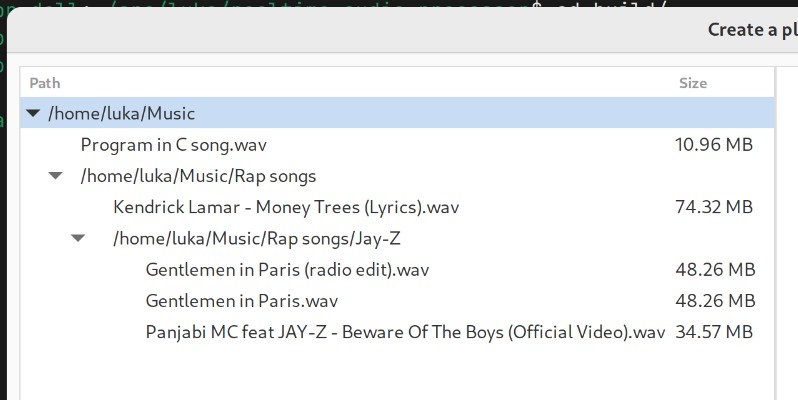
\includegraphics[width=13cm]{./file browser demo.png}
	\caption{Audio files are displayed in a graphical tree, backed by a tree in memory}
\end{figure}

\subsubsection{Tree data structure - \textit{include/data/tree.h}}
First, it was necessary to implement a tree data structure. Each node has a piece of data, followed by a list pointers to child nodes. Each child node may itself contain a piece of data, and a list of its own children.

As in C++ one must free explicit heap allocations manually,  recursion had to be used in the destructor. When the root node is destroyed, the following process occurs:
\begin{enumerate}
	\item C++ will call the destructor of the tree
	\item The tree iterates through all its children and calls their own respective destructors (line 16)
	\item This process repeats recursively until all children have deallocated their own children, and then finally themselves.
	\item Finally the root node deallocates itself.
\end{enumerate}
The full code is listed below.
\pagebreak
\inputminted[linenos]{c++}{../include/data/tree.h}

\pagebreak
\subsubsection{File Browser - \textit{src/ui/file\_browser.cpp}}
The file browser uses the tree data structure to store its files. Below are the relevant parts of the code, followed by a description.

\inputminted[linenos, firstline=47, lastline=108]{c++}{../src/ui/file_browser.cpp}

\paragraph{The \textit{ScanDirectory} subroutine} This function is called on the root audio file directory (the user's Music folder). It creates a tree with a single node, containing the path to this directory. It then iterates through all the files and folders in the root directory. Files are added as children of the root node. If a directory is encountered instead, a tree for that directory is created by recursively calling \textit{ScanDIrectory} again, which is then added as a child to the existing tree. In this way, all files and folders contained within the root directory are added.  

\paragraph{The \textit{AddDirectory} subroutine} This subroutine is called once the tree containing all files and folders has already been created in \textit{ScanDirectory}. Each element is recursively added to a \textit{wxTreeListCtrl} (for the purposes of displaying the tree in the GUI) by first adding the directory itself, followed by the files contained within, then adding the sub-directories, which is done by recursively calling the function.